\documentclass[11pt,compress,t,notes=noshow, aspectratio=169, xcolor=table]{beamer}

\usepackage{../../style/lmu-lecture}
% Defines macros and environments
% This file is included in slides and exercises

% Rarely used fontstyle for R packages, used only in 
% - forests/slides-forests-benchmark.tex
% - exercises/single-exercises/methods_l_1.Rnw
% - slides/cart/attic/slides_extra_trees.Rnw
\newcommand{\pkg}[1]{{\fontseries{b}\selectfont #1}}

% Spacing helpers, used often (mostly in exercises for \dlz)
\newcommand{\lz}{\vspace{0.5cm}} % vertical space (used often in slides)
\newcommand{\dlz}{\vspace{1cm}}  % double vertical space (used often in exercises, never in slides)
\newcommand{\oneliner}[1] % Oneliner for important statements, used e.g. in iml, algods
{\begin{block}{}\begin{center}\begin{Large}#1\end{Large}\end{center}\end{block}}

% Don't know if this is used or needed, remove?
% textcolor that works in mathmode
% https://tex.stackexchange.com/a/261480
% Used e.g. in forests/slides-forests-bagging.tex
% [...] \textcolor{blue}{\tfrac{1}{M}\sum^M_{m} [...]
% \makeatletter
% \renewcommand*{\@textcolor}[3]{%
%   \protect\leavevmode
%   \begingroup
%     \color#1{#2}#3%
%   \endgroup
% }
% \makeatother


\newcommand{\pih}{\fh}

\title{Interpretable Machine Learning}
% \author{LMU}
%\institute{\href{https://compstat-lmu.github.io/lecture_iml/}{compstat-lmu.github.io/lecture\_iml}}
\date{}

\newcommand{\gh}{\hat{g}}

\begin{document}

	
% Set style/preamble.Rnw as parent.

% Load all R packages and set up knitr

% This file loads R packages, configures knitr options and sets preamble.Rnw as 
% parent file
% IF YOU MODIFY THIS, PLZ ALSO MODIFY setup.Rmd ACCORDINGLY...

% Defines macros and environments

\newcommand{\titlefigure}{figure/lime5}
\newcommand{\learninggoals}{
	\item Understand motivation for LIME
	\item Develop a mathematical intuition}

\lecturechapter{LIME}
\lecture{Interpretable Machine Learning}

% Prerequisite: le-intro

% ------------------------------------------------------------------------------
\begin{frame}[c]{LIME}
\begin{itemize}
		\item Local Interpretable Model-agnostic Explanations (LIME) assume that even if a ML model is very complex, the local prediction can be described with a simpler model
		\smallskip\pause
		\item  LIME explains \textbf{individual} predictions of \textbf{any} black-box model by approximating the model \textbf{locally} with an interpretable model
		\smallskip\pause
		\item Called local surrogate models $\leadsto$ often inherently interpretable models such as linear models or classification/regression trees are chosen\\
		\smallskip\pause
		\item LIME should answer why a ML model predicted $\hat y$ for input $\xv$
		\smallskip\pause
		\item LIME is model-agnostic and can handle tabular, image and text data 
\end{itemize}
\end{frame}


\begin{frame}[c]{LIME: Characteristics}

    \textbf{Definition:}\\
	LIME provides a local explanation for a black-box model $\fh$ in form of a model $\gh \in \Gspace$ with $\Gspace$ as the class of potential (interpretable) models\\[2em]
	
	
	Model $g$ should have two characteristics:
	\begin{enumerate}
		\item \textbf{Interpretable}: relation between the input variables and the response are easy to understand  
		\item \textbf{Locally faithful / Fidelity}: similar behavior as $\fh$ in the vicinity of the obs. being predicted
	\end{enumerate}
	
	\vspace{2em}
	Formally, we want to receive a model $\gh$ with \textbf{minimal complexity and maximal local-fidelity} 
\end{frame}


\begin{frame}{Model Complexity}
    
    We can measure the complexity of a model $\gh$ using a complexity measure $J(\gh)$ \lz

 	\textbf{Example: Linear model}\\
 	\begin{itemize}
 	    \item Let $\Gspace = \left\{g: \Xspace \to \R ~|~g(\xv) = s(\thetab^\top \xv)\right\}$ be the class of linear models
 	    \item $s(\cdot)$: identity function for linear regression or logistic sigmoid function for logistic regression
 	    \item[$\leadsto$] $J(g) = \sum_{j = 1}^p \ind_{\{ \theta_j \neq 0 \}}$ could be the L$_0$ loss, i.e., the number of non-zero coefficients 
 	\end{itemize}
 	\lz\pause
 	
 	\textbf{Example: Tree}\\
 	\begin{itemize}
 	    \item Let $\Gspace = \left\{g:\Xspace \to \R ~|~g(\xv) = \sum_{m=1}^M c_m \ind_{\{ \xv \in Q_m \}}\right\}$ be the class of trees\\
 	     i.e., the class of additive models (e.g., constant $c_m$)  over the leaf-rectangles $Q_m$
 	    \item[$\leadsto$] $J(g)$ could measure the number of terminal/leaf nodes
 	\end{itemize}
 	
\end{frame}
 
\begin{frame}{Local model fidelity}
 	\begin{itemize}
 		\item $g$ is locally faithful to $\fh$ w.r.t. $\xv$ 
 		if for $\zv \in \Zspace \subseteq \R^p$ close to $\xv$, predictions of $\gh(\zv)$ are close to $\fh(\zv)$ 
 		\item In an optimization task: the closer $\zv$ is to $\xv$, the closer $\gh(\zv)$ should be to $\fh(\zv)$  
 		\pause
 		\item Two required measures:
 		\begin{enumerate}
 			\item A proximity (similarity) measure $\neigh(\zv)$ between $\zv$ and $\xv$, e.g. the exponential kernel:
 			$$\neigh(\zv) = exp(-d(\xv, \zv)^2/\sigma^2)$$ 
 			with $\sigma$ as the kernel width and $d$ as the Euclidean distance (numeric features) or the Gower distance (mixed features) 
 			\pause
 			\item A distance measure or loss function $L(\fh(\zv), \gh(\zv))$, e.g. the L$_2$ loss/squared error
 			$$L(\fh(\zv), \gh(\zv)) = (\gh(\zv) - \fh(\zv))^2$$ 
 		\end{enumerate}
 		\pause
 		\item Given points $\zv$, we can measure local fidelity of $g$ with respect to $\fh$ in terms of a weighted loss
 		$$ L(\fh, g, \neigh) = \sum_{\zv \in \Zspace} \neigh(\zv) L(\fh(\zv), \gh(\zv)) $$
 		%\item Note that identifying \textbf{locally} faithful explanations that are interpretable is less of a challenge than identifying \textbf{globally} faithful explanations. Yet, global fidelity implies local fidelity but not vice versa.
 	\end{itemize}
\end{frame}

\begin{frame}[c]{Minimization task}
	\begin{itemize}
		\item Optimization objective of LIME: 
		$$ \argmin_{g \in \Gspace} L(\fh, \gh, \neigh) + J(g)$$
		\item In practice:
		\begin{itemize}
		    \item LIME only optimizes $L(\fh, \gh, \neigh)$ (model-fidelity) 	
		    \item Users decide threshold on model complexity $J(g)$ beforehand
		\end{itemize}
		\item Goal: \textbf{model-agnostic} explainer
		\begin{itemize}
    		\item[$\leadsto$] optimize $L(\fh, \gh, \neigh)$ without making any assumptions about $\fh$ 
    		\item[$\leadsto$] learn $\gh$ only approximately  
		\end{itemize}
		\end{itemize}
\end{frame} 

\begin{frame}[c]{LIME Algorithm: Outline}
		
		\textbf{Input}:
		\begin{itemize}
		    \item Pre-trained model $\fh$
		    \item Observation $\xv$ whose prediction $\fh(\xv)$ we want to explain
		    \item Model class $\Gspace$ for local surrogate (to limit the complexity of the explanation)
		\end{itemize}
		
		\pause
		\medskip
		
		\textbf{Algorithm}:
		\begin{enumerate}
    		\item Independently sample new points $\zv \in \Zspace$ 
    		\item Retrieve predictions $\fh(\zv)$ for obtained points $\zv$ 
    		\item Weight $\zv \in \Zspace$ by their proximity $\neigh(\zv)$
    		\item Train an interpretable surrogate model $g$ on weighted data points $\zv \in \Zspace$\\ $\leadsto$ predictions $\fh(\zv)$ are the target of this model
    		\item Return the interpretable model $\gh$ as the explainer
		\end{enumerate}
		

	
\end{frame} 

\begin{frame}[c]{LIME Algorithm: Example}

    	\textbf{Illustration} of LIME based on a classification task:
		\begin{itemize}
			\item Light/dark gray background: prediction surface of a classifier
			\item Yellow point: $\xv$ to be explained
			\item $\Gspace$: class of logistic regression models 
		\end{itemize}
		\begin{center}
			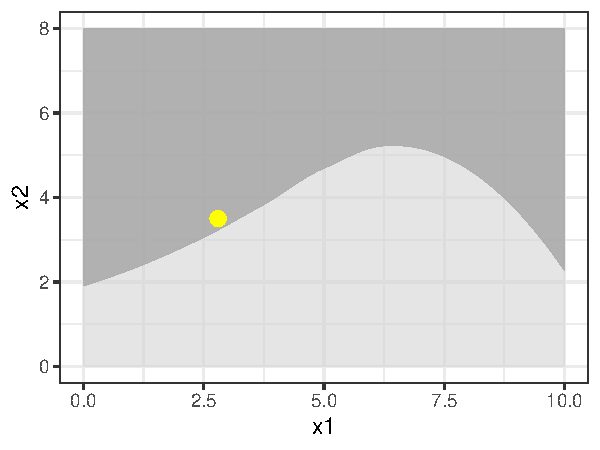
\includegraphics[width=0.35\textwidth]{figure/lime2}
		\end{center}

\end{frame} 


\begin{frame}[c]{LIME Algorithm: Example (Step 1+2: Sampling) \citebutton{Ribeiro. 2016}{https://github.com/marcotcr/lime}}
		
		Strategies for sampling: 
		\begin{itemize} 
			\item Uniformly sample new points from the feasible feature range 
			\item Use the training data set with or without perturbations
			\item Draw samples from the estimated univariate distribution of each feature
			\item Create an equidistant grid over the supported feature range  
		\end{itemize}
		\vspace{-.5cm}
		\begin{columns}
        \begin{column}{0.5\textwidth}  %%<--- here
            \begin{figure}
             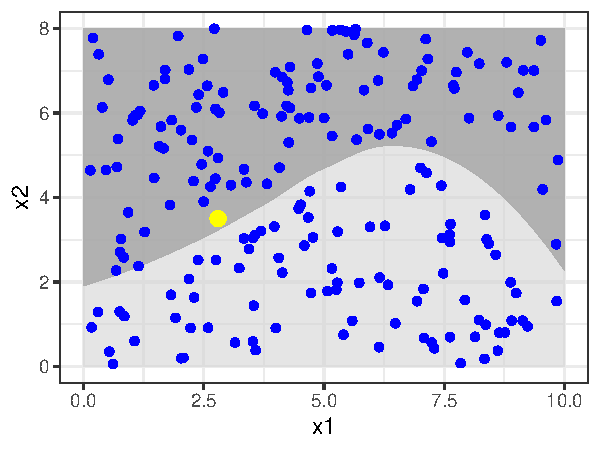
\includegraphics[width=.8\textwidth]{figure/lime3} 
             \vspace{-0.3cm}
             \caption{Uniformly sampled}
             \end{figure}
        \end{column}
        \begin{column}{0.5\textwidth}  %%<--- here
		    \begin{figure}
			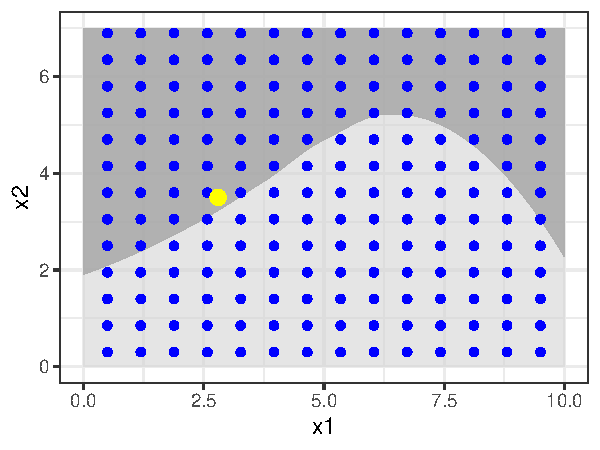
\includegraphics[width=.8\textwidth]{figure/lime3a}
			  \vspace{-0.3cm}
    		    \caption{Equidistant grid}
    		\end{figure}   
    \end{column}
\end{columns}
\end{frame}
		
\begin{frame}{LIME Algorithm: Example (Step 3: Proximity) \citebutton{Ribeiro. 2016}{https://github.com/marcotcr/lime}}

	In this example, we use the exponential kernel defined on the Euclidean distance $d$
		 $$\neigh(\zv) = exp(-d(\xv, \zv)^2/\sigma^2).$$ 
		\begin{center}
			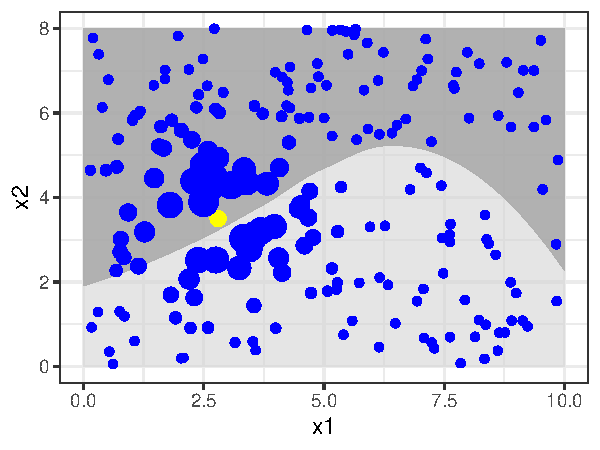
\includegraphics[width=0.4\textwidth]{figure/lime4}
		\end{center}
		
% MARIUS: Not relevant for the example; if we want to introduce it, we should do it somewhere else
% 	An alternative is the Gower proximity: 
% 	$\neigh(\zv) = 1 - \Gower(\zv, \xv) =  1 - \frac{1}{p}\sum_{j = 1}^{p} \delta_G(z_j, x_j) $ 
% 	$\textnormal{ with } \delta_G(z_j, x_j) = 
% 	\begin{cases}
% 	\frac{1}{\widehat{R}_j}|z_j- x_j| & \text{if $x_j$ and $z_j$ are numerical} \\
% 	\mathbb{I}_{z_j \neq x_j} & \text{if $x_j$ and $z_j$ are categorical}
% 	\end{cases}.$
		
\end{frame}
		
\begin{frame}[c]{LIME Algorithm: Example (Step 4: Surrogate) \citebutton{Ribeiro. 2016}{https://github.com/marcotcr/lime}}
		In our example, we fit a \textbf{logistic regression} model (consequently, $L(\fh(\zv), \gh(\zv))$ is the Bernoulli loss)
		\begin{center}
			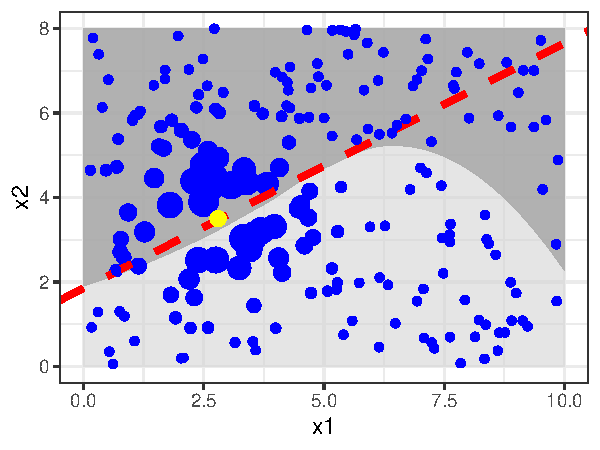
\includegraphics[width=0.4\textwidth]{figure/lime5}
		\end{center}
\end{frame}

\endlecture
\end{document}